%!TEX root = ../document.tex
\chapter{Broken Authentication and Session Management}
\label{BrokenAuthenticationAndSessionManagement}

\section{Erklärung}
Diese Sicherheitslücke befindet sich in dem OWASP Top 10 Risk Rating 2017 auf dem 2. Platz (OWASP A2). 
Auf vielen Web-Applikationen wird eine Benutzerauthentifizierung mit Benutzername und Passwort benötigt, um deren Dienste zu nutzen. Beispiele sind hierfür Online-Shops, Social-Media-Plattformen und Online-Banking. 
\\
Für die Interaktion zwischen dem angemeldeten Benutzer und der Web-Applikation ist das Session-Management nöig, wobei die gesammelten Session-Informationen in Cookies unter der eindeutigen Session-ID der Benutzer-Session abgespeichert werden. Cookies werden vom Browser verwendet, um client-seitig Informationen abzuspeichern.
\\
Der technische Hintergrund ist die Zustandslosigkeit des HTTP-Protokolls. Das HTTP-Protokoll wird für die Kommunikation zwischen dem Client und dem Web-Server eingesetzt. Die Zustandslosigkeit führt dazu, dass der Web-Server Seitenaufrufe unabhängig voneinander interpretiert und keinen Zusammenhang herstellen kann. Mit Hife des Session-Managements werden die Seitenaufrufe eines Benutzers in einer Session einander zugeordnet. Die Session-ID ist eine lange und zufällige Zeichenkette, wobei sichergestellt werden muss, dass dieser Identifier eindeitig ist und nicht leicht zu erraten ist.
\\
Mögliche Konsequenzen von Fehlern in der Authentifizierung und im Session-Management sind die Kompromittierung oder Übernahme von Benuzerkonten.

\subsection{Fehler in der Authentifizierung}
Wenn die Passwort-Policy für die Registrierung nicht ausreicehnd streng ist, können die Benutzer zu schwache Passwörter verwenden. Dadurch kann ein Brute-Force-Angriff ermöglicht werden, wobei durch systematisches Probieren aller möglichen Kombinationen die Benutzernamen und dazugehörigen Passwörter fremder Benutzer erraten werden können.\\
Eine weitere Fehlerquelle ist die Verschlüsselung von Benutzername und Passwort. Wenn diese Daten im Klartext über das HTTP-Protokoll versendet werden, kann ein Angreifer die Kommunikation abhören. Wenn beim Abspeichern der Benutzerdaten auf das Hash-Verfahren bzw. Verschlüsselung verzichtet wird, sind diese Daten ungeschützt vor anderen Sicherheitslücken wie z.B. SQL-Injections.\\
Auch wenn der Web-Server aussagekräftige Informationen über bereits bestehende Benutzerkonten Preis gibt, kann ein fremdes Benutzerkonto übernommen werden. Bei der Konto-Erstellung oder "Passwort-Zurücksetzen"-Funktion kann ggf. ein bestehender Benutzername ermittelt werden. Der Benutzername stellt bereits die erste Hälfte der Lösung des Benutzername-Passwort-Rätsels dar.

\subsection{Fehler im Session-Management}
Die Wahl der Session-ID können nicht ausreichend zufällig gestaltet sein, so dass eine gültige Session-ID erraten werden kann. Wenn zudem die Session-ID als Parameter in der URL übergeben wird, kann eine Session von einem Dritten übernommen werden. Dieser Dritte kann dadurch alle Funktionen der Web-Applikation mit den Berechtigungen des angemeldeten Benutzers verwenden. Wenn die URL unverschlüsselt übertragen wird, kann ein Angreifer ebenfalls eine fremde Session-ID ermitteln und diese Session eines angemeldeten Benutzers übernehmen. Das HTTPS-Protokoll bietet eine Verschlüsselung für diese Problematik.\\
Wenn Session-IDs nach dem Abmelden eines Benutzers nicht ungültig gesetzt werden, können diese zur WIederherstellung der Anwender-Session missbraucht werden. Auch wenn sich die Session-IDs nicht mit erneuter Anmeldung ändern, werden diese zu vorhersehbar für neue Anmeldungen.\\
Wenn das HttpOnly-Attribut nicht gesetzt wird, wird das Auslesen des Session-Cookies über Skriptsprachen ermöglicht. Im Rahmen eines XSS-Angriffs kann die Session-ID eines anderen Benutzers ermittelt werden. 

\subsection{Gegenmaßnahmen}
Die Authentifizierungsfunktion sollte so gestaltet sein, dass nach wiederholter Fehleingabe der Anmeldedaten das Benutzerkonto oder die Aufrufer-IP temporär gesperrt werden.\\
Außerdem sollte weder bei der Registrierung noch bei der "Passwort-Vergessen"-Funktion eine aussagekräftige Rückmeldung über bereits existierende Benutzernamen gegeben werden. Wenn dies aus Gründen der Benutzerfreundlichkeit nicht möglich ist, sollten zumindest automatisierte Abfragen unterbunden werden.\\
Die Übermittlung der Anmeldedaten sollte ausschließlich verschlüsselt mit TLS und die Speicherung der Passwörter in gehashter Form mit geeigneten kryptographischen Funktionen gestaltet werden.\\
Session-IDs sollten ausreichen zufällig gewählt, nicht unverschlüsselt übertragen und bei einer Abmeldung serverseitig beendet werden. Zum Erzwingen der Verschlüsselten Übertragung der Session-ID kann das Secure-Attribut des Session-Cookies aktiviert werden. Außerdem sollte das HttpOnly-Attribut gesetzt werden, um ein Auslesen des Cookies mittels JavaScript zu verhindern.\\
Um Session-Übernahmen zu vermeiden, können darüber hinaus die Session des Anwenders mit spezifischen Nutzermerkmalen, beispielsweise dem entsprechenden User-Agent oder der IP-Adresse verknüpft werden.\\
Neben diesen Standardmaßnahmen sollten auch die von der OWASP formulierten Anforderungen an Authentifizierung und Session-Management umgesetzt werden. Diese sind in den OWASP Application Security Verification Standards beschrieben.\\
\\
Quelle:\\ https://www.datenschutz-notizen.de/owasp-top-ten-a2-fehler-in-authentifizierung-und-session-management-2713238/

\section{Übungen}
\textbf{Registrierung}\\
Das Lernziel der 1. Übung Registrierung ist es, dem Anwender gängige Passwortregeln zu zeigen. Inhalt der Übung ist es, sich erfolgreich zu registrieren, d.h. man muss die Passtwortregeln einhalten.

\begin{figure}[H]
	
	\centering
	
	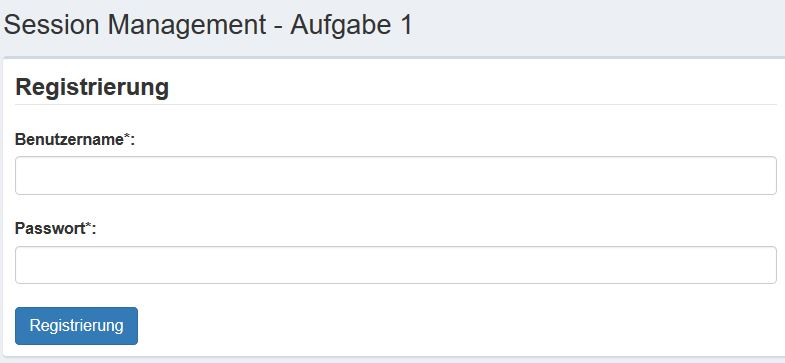
\includegraphics[width=1.0\linewidth]{images/BrokenAuthenticationAndSessionManagement/Registrierung_Start}
	
	\caption[Registrierung]{Registrierung mit gängigen Passwortregeln}
	
	\label{fig:Aufgabe 1 Registrierung}
	
\end{figure}
Für dieses Übung werden zwei Hinweise zur Verfügung gestellt. Der erste Hinweis ist, dass man sich an die allgemein üblichen Regeln halten sollte, damit man sich registrieren kann. In dem zweiten Hinweis werden die verwendeten Passwortregeln aufgelistet: mind. 8 Zeichen lang sein, einen Großbuchstaben, einen Kleinbuchstaben und eine Zahl. \\
Wenn man sich dann erfolgreich registriert hat, wird man zu folgender Seite weitergeleitet:\\
\begin{figure}[H]
	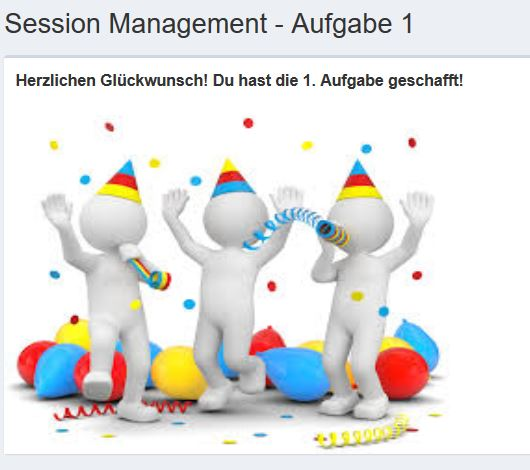
\includegraphics[width=1.0\linewidth]{images/BrokenAuthenticationAndSessionManagement/Registrierung_Ende}
	\caption[Registrierung]{Landing-Page nach erfolgreicher Registrierung}
	\label{fig:Aufgabe 1 Abschluss}
\end{figure}
\textbf{Login}\\
Die zweite Übung hat das Ziel, aufzuzeigen, wie leicht Passwörter zu erraten sind, wenn die gängigen Paswortregeln nicht eingehalten werden müssen. Es gibt sehr beliebte und einfache Benutzername- und Paswort-Kombinationen, die man in dieser Übung ausnutzen kann.\\ 
Die Aufgabenstellung ist deshalb, sich mit einem fremden, unbekannten Benutzerkonto anzumelden. Dabei muss man Benutzername und Passwort erraten. \\
\begin{figure}[H]
	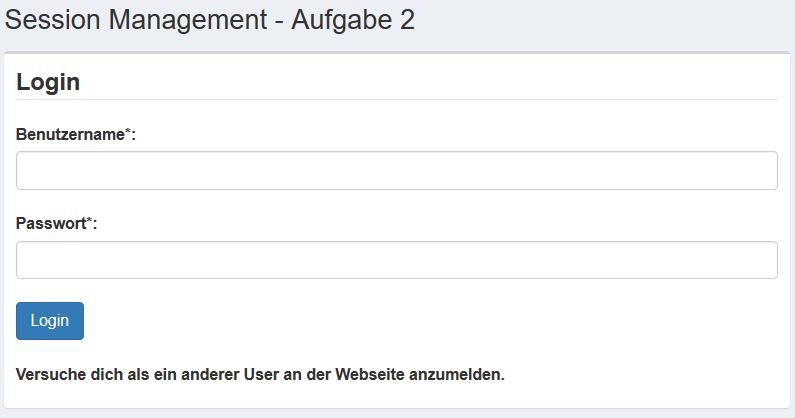
\includegraphics[width=1.0\linewidth]{images/BrokenAuthenticationAndSessionManagement/Login_Start}
	\caption[Login]{Aufgabe 2 Login}
	\label{fig:Aufgabe 2 Login}
\end{figure}
Dabei werden zwei Hinweise bei Bedarf gegeben. Der erste Hinweis ist, dass es sich hier um sehr einfache, beliebte Benutzernamen und Passwörter handelt. Wenn dieser Tipp nicht ausreicht, wird im zweiten Hinweis ein existierendes Paswort ('admin') gegeben. Zu diesem Benutzername würde das Passwort 'admin' passen. Es gibt jedoch auch andere Kombinationen: z.B. Benutzername 'benutzer' und als Passwort 'passwort1' oder 'fußballfan' und 'schalke04'.\\
Einige dieser beliebten Benutzernamen und Passwörter sind in der Datenbank der Webseite hinterlegt.\\
Wenn man sich dann erfolgreich mit einem fremden Benutzerkonto angemeldet hat, gelangt man zur letzten Seite der Übung:
\begin{figure}[H]
	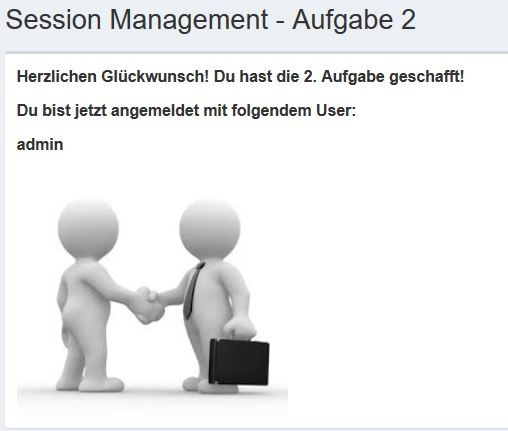
\includegraphics[width=1.0\linewidth]{images/BrokenAuthenticationAndSessionManagement/Login_Ende}
	\caption[Login]{Landing-Page nach erfolgreichem Login}
	\label{fig:Aufgabe 2 Abschluss}
\end{figure} 
Wenn man Benutzername und Passwort erraten hat, könnte man  die Funktionen mit den Berechtigungen des fremden Benutzerkontos nutzen. In unserer Übung wird das jedoch nicht mehr abgefragt.\\\\
\textbf{Logout}\\
Das Lernziel der dritten Übung ist es, dass beim Logout die Session zwingend beendet werden muss und die dazugehörigen Daten nicht mehr verfügbar sein dürfen.\\
Die Aufgabenstellung ist, sich nach dem Logout ohne erneute Anmeldung zurück zu der Webseite als angemeldeter Benutzer zu gelangen.\\ 
\begin{figure}[H]
	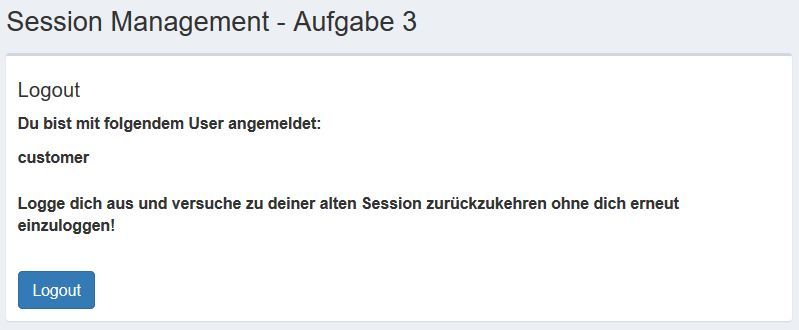
\includegraphics[width=1.0\linewidth]{images/BrokenAuthenticationAndSessionManagement/Logout_Start}
	\caption[Logout]{Aufgabe 3 Logout}
	\label{fig:Aufgabe 3 Logout}
\end{figure}
Über den Logout-Button wird man ausgeloggt und wird zu Logout-Seite weitergeleitet:
\begin{figure}[H]
	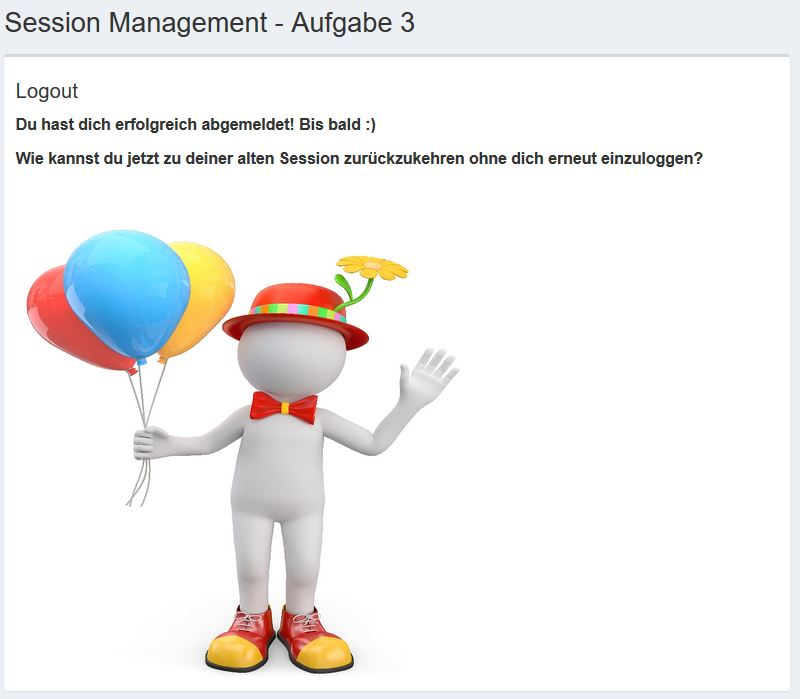
\includegraphics[width=1.0\linewidth]{images/BrokenAuthenticationAndSessionManagement/Logout_Mitte}
	\caption[Logout]{Logout-Seite}
	\label{fig:Aufgabe 3 Abschluss}
\end{figure}
Hier wird der Hinweis, dass der Browser eine 'zurück'-Funktion bietet, bei Bedarf zur Verfügung gestellt.\\
Wenn man diese nutzt, gelangt man wieder zur Startseite der Übung als angemeldeter Benutzer. Somit ist die Übung erfolgreich absolviert.\\\\
\textbf{URL-Manipulation}\\
Mit dieser letzten Übung soll gezeigt werden, dass man Session-Attribute und die Session-ID nicht sichtbar sein sollten, wie z.B. in der URL. Zudem darf die Session-ID nicht so spechend wie z.B. der Benutzername sein, sondern muss eine willkürliche Zeichenfolge sein.\\
Die Aufgabenstellung ist das Benutzerkonto des Admins zu übernehmen. Aktuell ist man mit dem Benutzer 'customer' angemeldet.\\
\begin{figure}[H]
	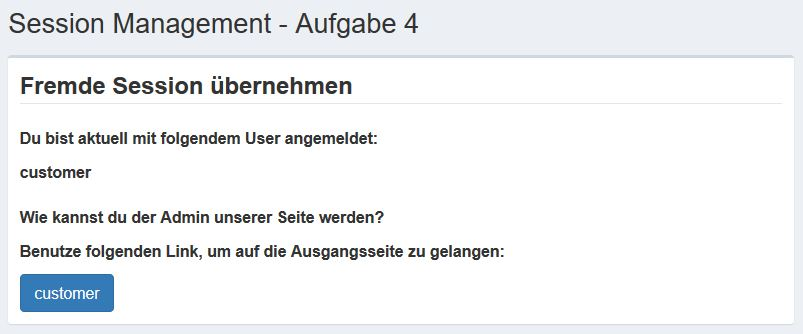
\includegraphics[width=1.0\linewidth]{images/BrokenAuthenticationAndSessionManagement/URL_Start}
	\caption[URL]{Aufgabe 4 URL-Manipulation}
	\label{fig:Aufgabe 4 URL-Manipulation}
\end{figure}
Wenn man den Button 'customer' betätigt, gelangt man zur Ausgangsseite:
\begin{figure}[H]
	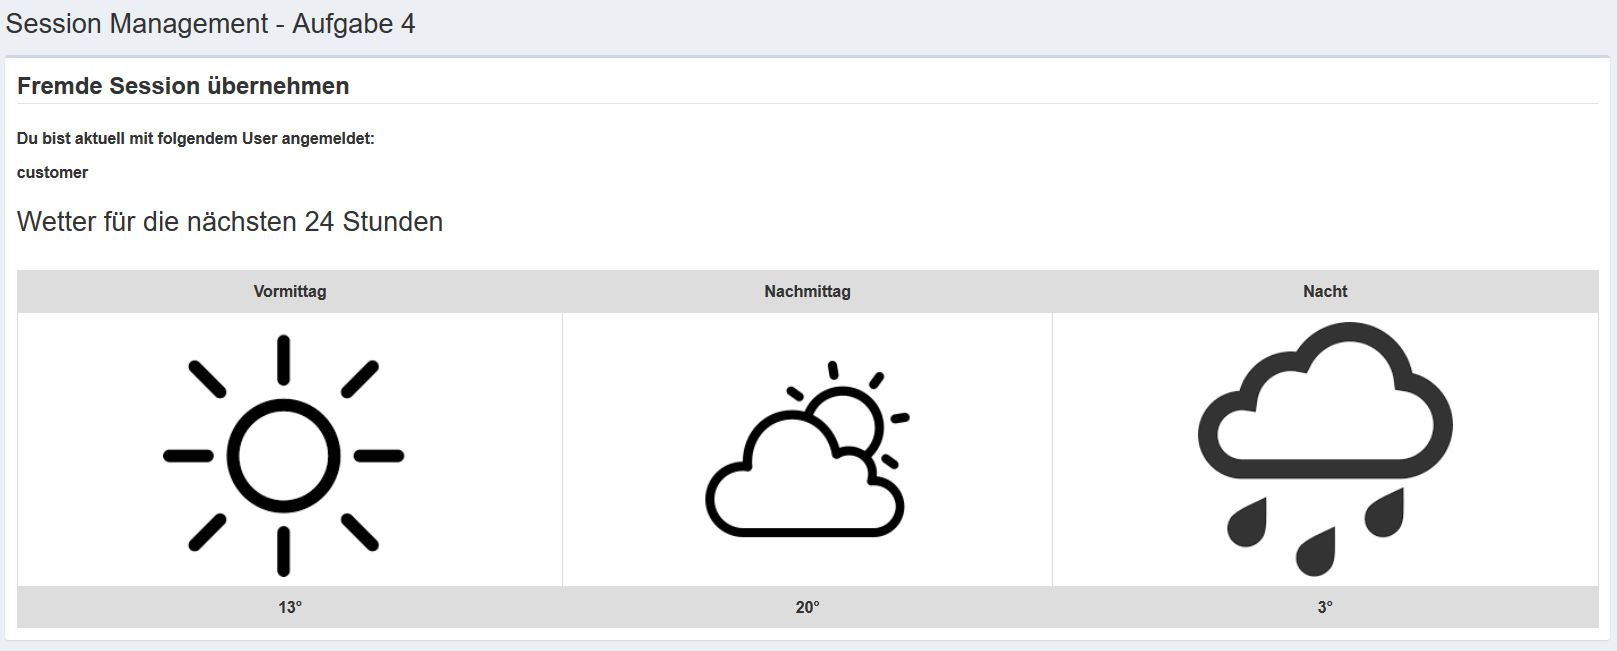
\includegraphics[width=1.0\linewidth]{images/BrokenAuthenticationAndSessionManagement/URL_customer}
	\caption[URL]{Aufgabe 4 Ausgangsseite des Customers}
	\label{fig:Aufgabe 4 Ausgangsseite des Customers}
\end{figure}
Auf der Ausgangsseite werden zwei Hinweise angeboten. Der erste Tipp, weißt auf die Unterschiede des GET- und POST-Requests des HTTP-Protokolls hin. Der zweite Tipp lenkt die Aufmerksamkeit des Anwenders auf die Parameter der URL, die man manipulieren kann.\\
Die Parameter in der URL sind auch der Lösungsweg, da hier der Username hinterlegt ist.
\begin{figure}[H]
	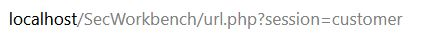
\includegraphics[width=1.0\linewidth]{images/BrokenAuthenticationAndSessionManagement/URL_customer_url}
	\caption[URL]{Aufgabe 4 URL der Ausgangsseite des Customers}
	\label{fig:Aufgabe 4 URL der Ausgangsseite des Customers}
\end{figure} 
Wenn man den Wert des Parameters 'session' auf 'admin' ändert, gelang man zur Session des Admins.
\begin{figure}[H]
	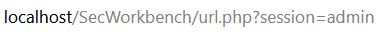
\includegraphics[width=1.0\linewidth]{images/BrokenAuthenticationAndSessionManagement/URL_admin_url}
	\caption[URL]{Aufgabe 4 URL der Ausgangsseite des Admins}
	\label{fig:Aufgabe 4 URL der Ausgangsseite des Admins}
\end{figure}
Der Admin kann den Wetterbericht der nächsten drei Tage sehen, der Kunde jedoch nur das Wetter der nächsten 24 Stunden. Wenn man auf dieser Seite angelangt ist, hat man die letzte Übung erfolgreich abgeschlossen.
\begin{figure}[H]
	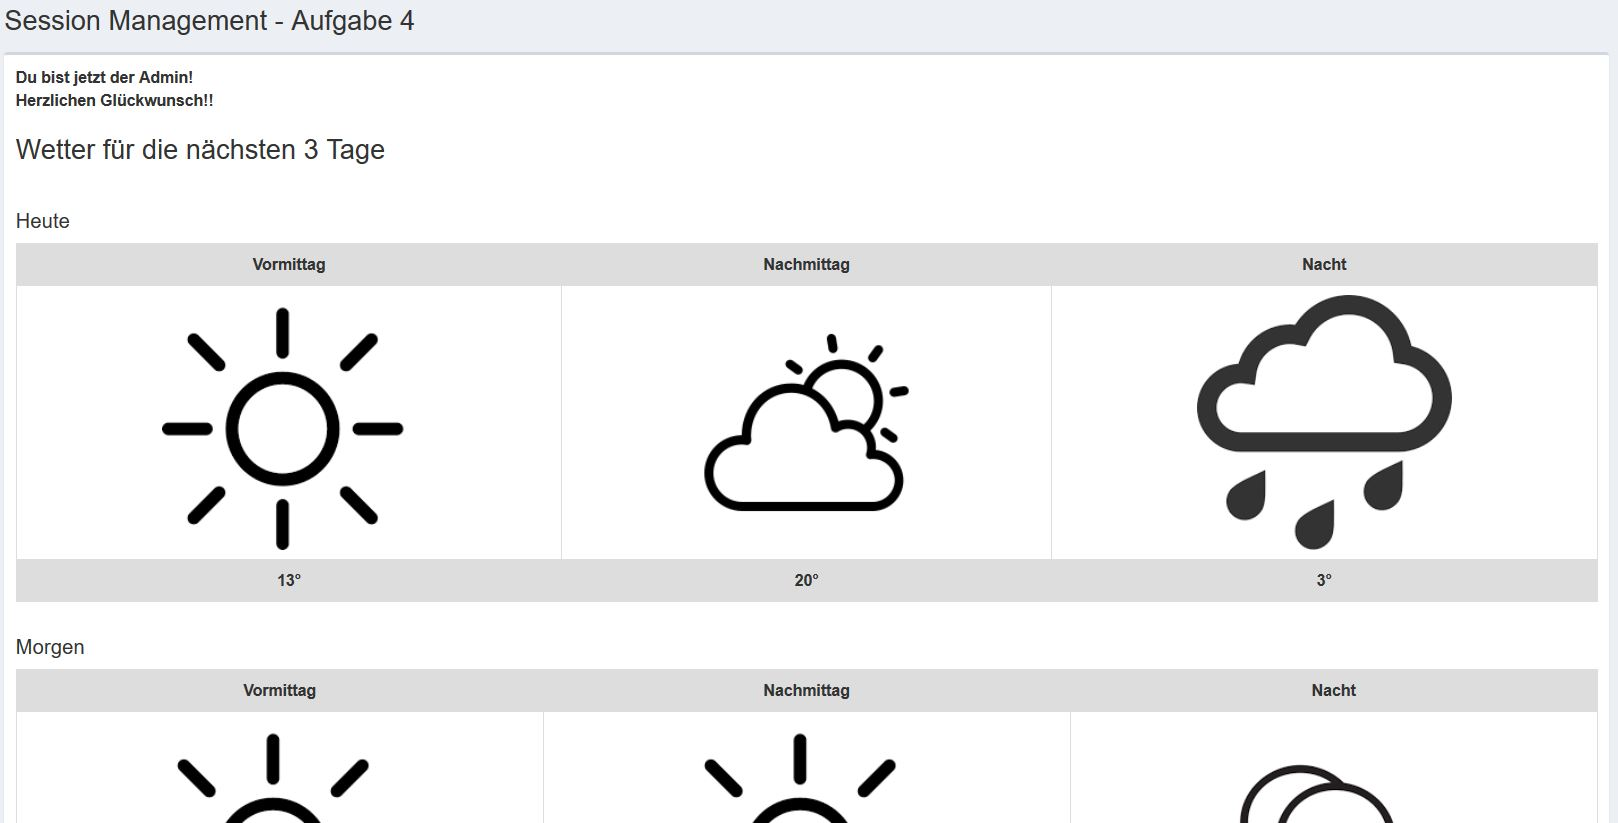
\includegraphics[width=1.0\linewidth]{images/BrokenAuthenticationAndSessionManagement/URL_admin}
	\caption[URL]{Aufgabe 4 Ausgangsseite des Admin}
	\label{fig:Aufgabe 4 Ausgangsseite des Admin}
\end{figure}